\documentclass[11pt]{article}
\usepackage{./EllioStyle}
\usepackage{listings}
\usepackage{multicol}
\usepackage{forest}

\definecolor{codegreen}{rgb}{0,0.6,0}
\definecolor{codegray}{rgb}{0.5,0.5,0.5}
\definecolor{codepurple}{rgb}{0.58,0,0.82}
\definecolor{backcolour}{rgb}{0.95,0.95,0.92}

\lstdefinestyle{mystyle}{
%    backgroundcolor=\color{backcolour},   
    commentstyle=\color{codegreen},
    keywordstyle=\color{magenta},
    numberstyle=\tiny\color{codegray},
    stringstyle=\color{codepurple},
    basicstyle=\ttfamily\footnotesize,
    breakatwhitespace=false,         
    breaklines=true,                 
    captionpos=b,                    
    keepspaces=true,                 
    numbers=left,                    
    numbersep=5pt,                  
    showspaces=false,                
    showstringspaces=false,
    showtabs=false,                  
    tabsize=2
}

\title{Learning Diabetes Ratios using Reinforcement Learning}
\author{Elliott Pryor}
\date{14 December 2021}

\rhead{Learning Diabetes Ratios using Reinforcement Learning}

\begin{document}
\maketitle


\section{Problem Statement}
The goal of this project is to explore machine learning options for medical data, specifically diabetes data.
Diabetes, specifically Type 1 diabetes, is a notoriously hard disease to manage.
There are seemingly countless variables that can influence blood sugar, and it is hard to keep track of all the information.
Lifelong diabetics can struggle to effectively manage their blood sugar. 
I am also a diabetic and experience these first-hand. This is an area that I am personally very invested in.
The purpose of this project is to explore potentially viable methods, specifically in reinforcement and transfer learning, for diabetes based problems. 
Transfer learning has led to great advances in computer vision and natural language processing, so it would be interesting to see if it is feasible to apply it in this area. 

The general outline is to use reinforcement learning on a simulated patient.
The reinforcement learner is hopefully able to learn how to adjust carbohydrate and basal ratios based on simulated outcomes.
A general model will be trained on a large set of patients. 
Then I hypothesize that this model can then be fine-tuned on a smaller amount of individual patient data in order to produce an individualized model for that patient.

\section{Diabetes Background}
Type 1 Diabetes (T1D) is a chronic health condition caused from pancreatic beta cell dysfunction and insulin depletion \cite{tyler2020artificial}.
In this work, we consider patients using the popular insulin-pump based therapy to manage insulin levels. 
Diabetes is a complicated disease to manage. 
At a high level, the patient is not able to produce insulin on their own, which influences blood glucose levels (BG).
The insulin pump manages blood sugar in three primary ways.

\begin{enumerate}
    \item Basal. The basal insulin is a constant amount of insulin administered continuously throughout the day.
    The purpose of basal insulin is to counteract the normal amount of glucose added to the blood throughout the day by the liver.
    If the basal rate is set correctly, the patient's BG should remain constant when no carbohydrates are consumed

    \item Carb. The carbohydrate-insulin ratio is used to counteract the rise in blood sugar caused by consuming carbohydrates. 
    This insulin is administered all at once (unlike basal). This is called a meal bolus.
    The amount of insulin administered in a bolus is given by the equation:
    $insulin = \frac{\text{carbohydrate intake}}{carb}$

    \item Correction. The correction ratio (not considered in this work) is used to adjust BG throughout the day. 
    If the patient's BG is too high it administers a correction bolus to bring the blood sugar down to targeted levels.
    The amount of insulin administered in a bolus is given by the equation:
    $insulin = \frac{\text{Current BG} - \text{Target BG}}{correction}$

\end{enumerate}

The general assumption is that these ratios remain fairly constant throughout a day, but they can vary over time.
Causes of variation include: metabolic changes (aging, illness, pregnancy, other) and changes in lifestyle (diet, amount of exercise, etc.).
The goal of this research is to create a model that can help inform the patient if they need to increase or decrease these ratios on average.


\section{Related Work}
One of the main starting points for related work is a survey paper written by Nichole Tyler and Peter Jacobs \cite{tyler2020artificial}.
This work provides a strong background in existing methods that have been applied to a variety of type 1 diabetes related problems.
This was largely my jumping off point for exploring methods that have been applied.
Recently, most of the work is on intelligently optimizing the amount of insulin given in a single meal bolus. 
This area is of practical significance given the predominance of insulin-pump therapy 
and the development of closed-loop systems that are designed to automatically administer insulin.
One common theme with these methods was noticed, they assume that a roughly correct basal-insulin rate and carbohydrate-insulin ratio are defined.
However, this is often not the case, which motivates this work. 
If we can determine the optimal base settings for basal and carb, we can improve the overall efficacy of these other algorithms as well throughout a day.

Zhu et. al. create an actor-critic method very similar to the proposed project.
However, along with most related work, this method is designed to recommend the amount of insulin to give at a single meal bolus \cite{zhu2020insulin}. 
The method used by the authors here motivated the initial investigation into using actor-critic methods. 

Due to the reinforcement learning framework that is being used, a simulation environment is needed for the agent to interact with.
There are several simulation environments. 
The primary environment is produced by UVA and Padova University which is FDA approved \cite{man2014uva}.
However, there is no available implementation of this.
So a simulation crated by Resalat et. al. was used which has an open-source MATLAB implementation \cite{resalat2019statistical}.
This solves a set of differential equations to model insulin dynamics within the body given carbohydrate intake and carb, basal insulin ratios.
This model also has 99 different patients, so it is possible to compare dynamics on different patients.


\section{Experimental Approach}
Using the model by Resalat et. al. \cite{resalat2019statistical} the agent is able to interact with the environment.
The agent recommends to either increase, decrease, or not to change the carbohydrate and basal rates, which are passed into the simulator. 
The simulator then returns the BG values at 5 minute intervals throughout the day.
This time-period was chosen because that is how often most continuous glucose monitors, like Dexcom, return BG values.
The reward is computed using the function in Equation \ref{eq:reward}.
Where $g_t$ is the glucose value at a given point in time, and $r_i$ is the reward for that individual glucose value.
This is essentially a numerically approximated weighted integral.
The values for $r_i$ were set based on work by Zhu et. al. \cite{zhu2020insulin}.

\begin{equation}
    R(G) = \sum_{g_t \in G} r_i, \quad r_i = \begin{cases}
        0.5 & 70 \leq g_t \leq 180 \\
        -0.8 & 180 < g_t < 300 \\
        -1 & 300 < g_t < 400 \\
        -1.5 & 55 < g_t < 70 \\
        -2 & \text{Otherwise}
    \end{cases}
    \label{eq:reward}
\end{equation}

The inputs into the models were the sequence of observed $g_t$ values as well as the current basal and carb ratios.
This produces an input vector of size 291. 
Several experiments were run with the Actor-Critic method reducing the dimensionality which had little effect on performance.

For most trials, models were trained on: 150 iterations on one patient, 500 iterations on one patient, 150 iterations over 50 patients, and 1000 iterations over 50 patients.
In these last two, the carbohydrate intake is also variable. 
We then compare the performance of different learning strategies as well as different checkpoints.

\subsection{Actor Critic}
I implemented the actor critic learning framework using pytorch. 
This is a policy gradient method. 
The critic takes output from the actor as well as the current state and attempts to predict the reward.
The actor takes current state information nad attempts to predict an action.
The outputs from the critic are used to train the critic model, as well as the actor model. 

For my expriments, I used several network architectures.
I first used a simple single linear layer (no hidden layers) for both the actor and critic.
I then used a single hidden layer in the critic of size 500, and 2 hidden layers in the actor both of size 500.
Relu was the activation function that was used on each layer, except the outputs of the actor which use a softmax function.

\subsection{Q-Learning}
I implemented Deep Q-Learning with memory replay in pytorch. 
Deep Q-Learning seems to be a very popular reinforcement learning algorithm, based on various articles and blog posts.
The advantage of Q-Learning is that it allows for memory replay because it is off-policy.
The original author state 
``Note that when learning by experience replay, 
it is necessary to learn off-policy (because our current parameters are different to those used to 
generate the sample), which motivates the choice of Q-learning.'' \cite{mnih2013playing}
Memory replay allows the model to be trained significantly more quickly and improves stability. 
The (state, action, next state, reward) 4-ples are stored in the memory and then sampled from when training.

The Q learning algorithm updates using the following equation:
$$Q_t(s,a) = Q_{t-1}(s, a) + \alpha \left[ R(s,a) + \gamma * \max_{a' \in A} Q_{t-1}(s', a') - Q_{t-1}(s,a) \right]$$
Where $\alpha$ is the learning rate, $R$ is the observed reward, $s'$ is the next state.

This was applied to two different network architectures:
\begin{enumerate}
    \item Two fully connected hidden layers in the both of size 500.
    \item Two 1D convolutional layers with kernel size = 5 for the glucose value inputs. 
    The output of this is flattened and the current insulin and carb ratios are concatenated, 
    and one fully connected hidden layer of size 128 is used to make final prediction.
    The convolutional layers are supposed to learn the glucose trends and patterns, while the last hidden layer uses the patterns and current ratios to select the action.
\end{enumerate}

$\gamma$ was also set to different values: $0.99, 0.5$.

\subsection{SARSA}
I implemented the SARSA algorithm with eligibility traces.
This is very similar to Q-Learning but is on-policy, so we cannot use memory replay. 
The only difference between SARSA and Q-Learning is we do not learn using the max action every time. 
Instead the update rule is:
$$Q_t(s,a) = Q_{t-1}(s, a) + \alpha \left[ R(s,a) + \gamma * Q_{t-1}(s', a') - Q_{t-1}(s,a) \right]$$
Where $a'$ is the next action that we will take (chosen using some policy derived from $Q$, which in our case is a decaying $\epsilon$-greedy).

The eligibility traces algorithm is implemented as in my notes from CSCI446 Spring 2020 as seen in Figure \ref{fig:sarsa}.
\begin{figure}[h] 
    \centering
    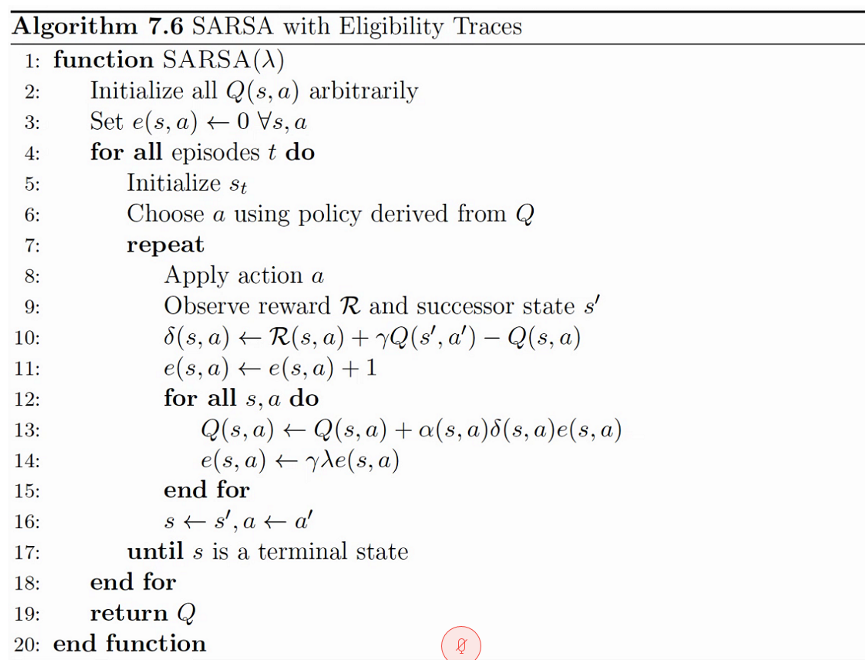
\includegraphics[width=0.55 \linewidth]{SARSA.png}
    \caption{SARSA with eligibility traces from lecture notes}
    \label{fig:sarsa}
\end{figure}

I implemented only the first network architecture from in Q-Learning (I did not implement the CNN), and set $\gamma = 0.99$, $\lambda = 0.8$.

\section{Results}
The results were not what I hoped for.
The actor critic methods were not able to successfully learn. 
They often just performed a random walk and had rewards of $<-200$ which is effectively killing the patient.

The Q-Learning and SARSA methods performed better.
For the very basic case, one patient with constant carb intake, the Q-learning methods converged to a decent solution.
One very strange phenomenon is that it did not converge to the best solution, or even the best seen solution.
It appears to get stuck in a local optimum and does not further explore the space. 

Models were evaluated using patient number 95 that was not seen during the training. 
The best action with the highest value was taken from the current state ($a = argmax_{a \in A} Q(a, s)$).
This was run for a total of 100 iterations to allow the model to converge, and to study how the model improves over time.
The model did not learn during this period, but was just allowed to increment and decrement the basal and carb ratio until it remained fairly constant.
Results are shown in Figure \ref{fig:all_results}.

Interestingly the standard neural network performed the best on the base case and the random 1000 trial.
The base case makes sense given that the state space is constant (one basal, carb pair maps to one blood glucose trend).
This does not hold in the random experiments as the glucose values depend on the random patient and the random carbohydrate intake.
So the standard neural network should be able to learn the rewards just by memorizing the states.
But on the random case, even fairly related states will have different glucose values,
so the standard neural net should not be able to correlate the states. 
This is part of what motivated investigating the cnn architecture. 
The most surprising aspect of this is that the standard neural network performed nearly optimal.
The maximum score possible is $144.5$. 
This is the score that is achieved on many different simulated `days'. 
So not only was the model able to interpret trends in glucose value, but it was able to converge the optimal solution,
which is something none of the other models ever did.

The universally poor performance on the random 150 training scheme is probably indiciative that there was not enough iterations to successfully train the model.
All of the models performed quite poorly. 
It is interesting that in all three schemes many models get stuck in some optimum with reward about -100.
Via inspection, this appears to have the basal and carbohydrate values at their minimum.
So the model learned to always reduce both basal and carb. 
While not ideal, this is preferred over increasing both, as too much insulin causes hypoglycemia which can be fatal,
while too little insulin has less acute health effects.
But in general, given that many of the models universally converge to this minimum, 
it is safe to say that the models are not learning very well.

\begin{figure}
    \centering

    \begin{subfigure}{0.62 \textwidth}
        \centering
        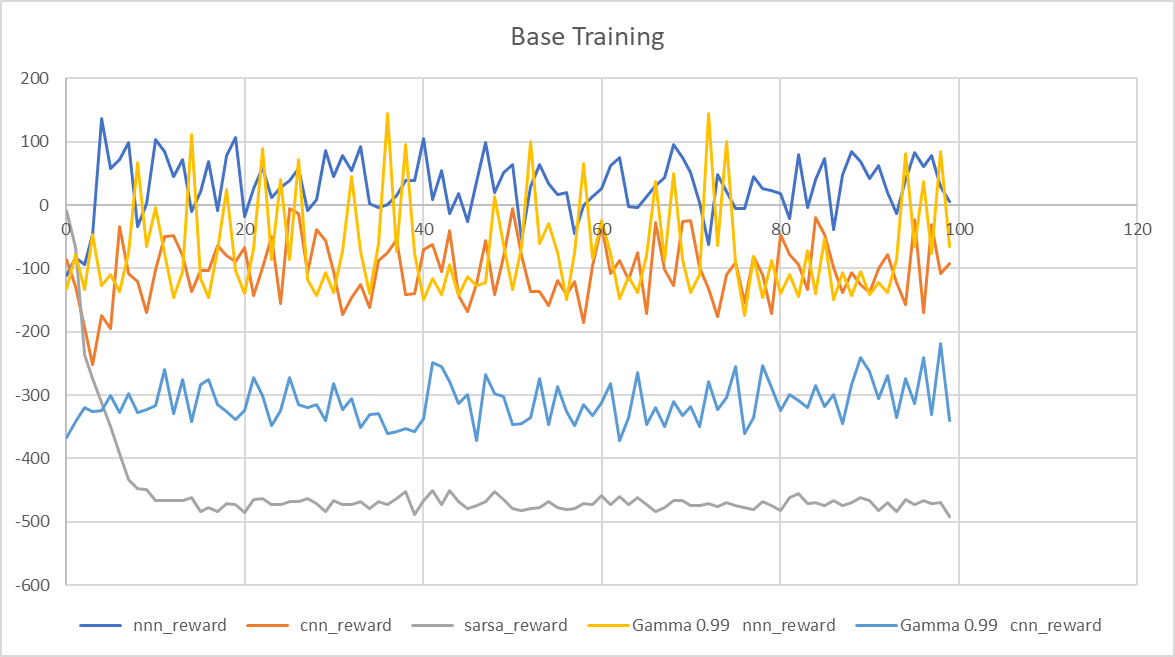
\includegraphics[width=\textwidth]{base.png}
        \caption{Evaluation of models using base training scheme. One patient, constant carb intake, for 150 iterations}
        \label{fig:base}
    \end{subfigure}
    
    \begin{subfigure}{0.62 \textwidth}
        \centering
        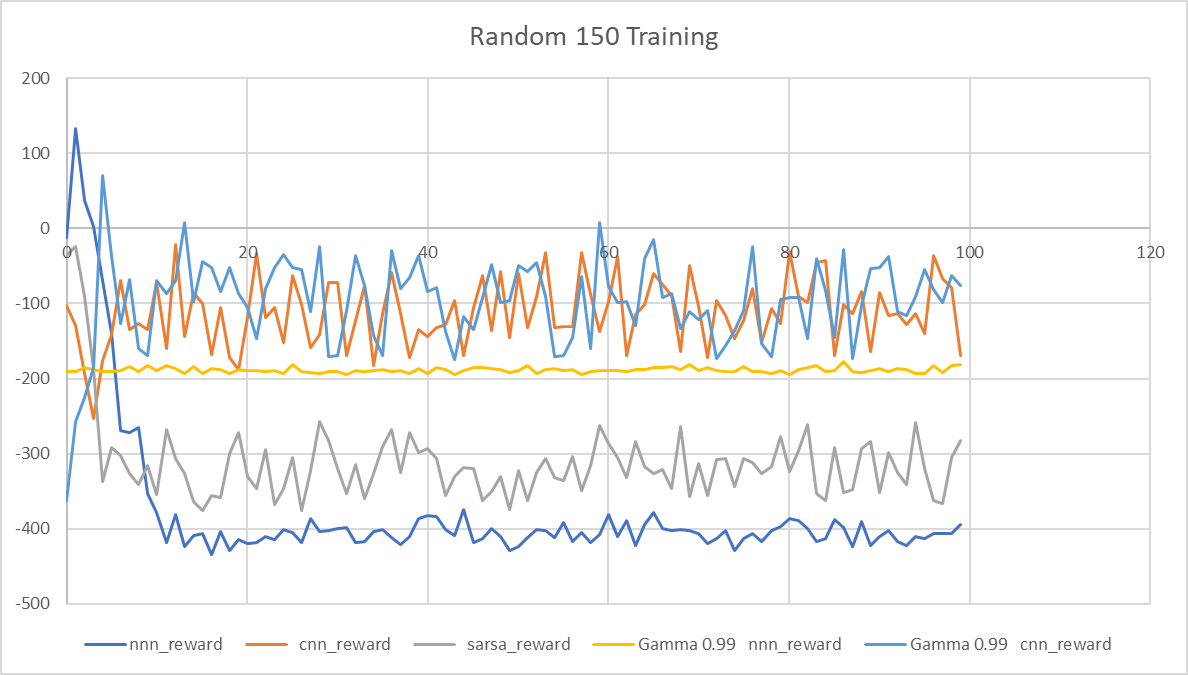
\includegraphics[width=\textwidth]{rand150.png}
        \caption{Evaluation of models using rand 150 training scheme. 50 patients randomly changed, variable carb intake, for 150 iterations}
        \label{fig:rand150}
    \end{subfigure}
    
    \begin{subfigure}{0.62 \textwidth}
        \centering
        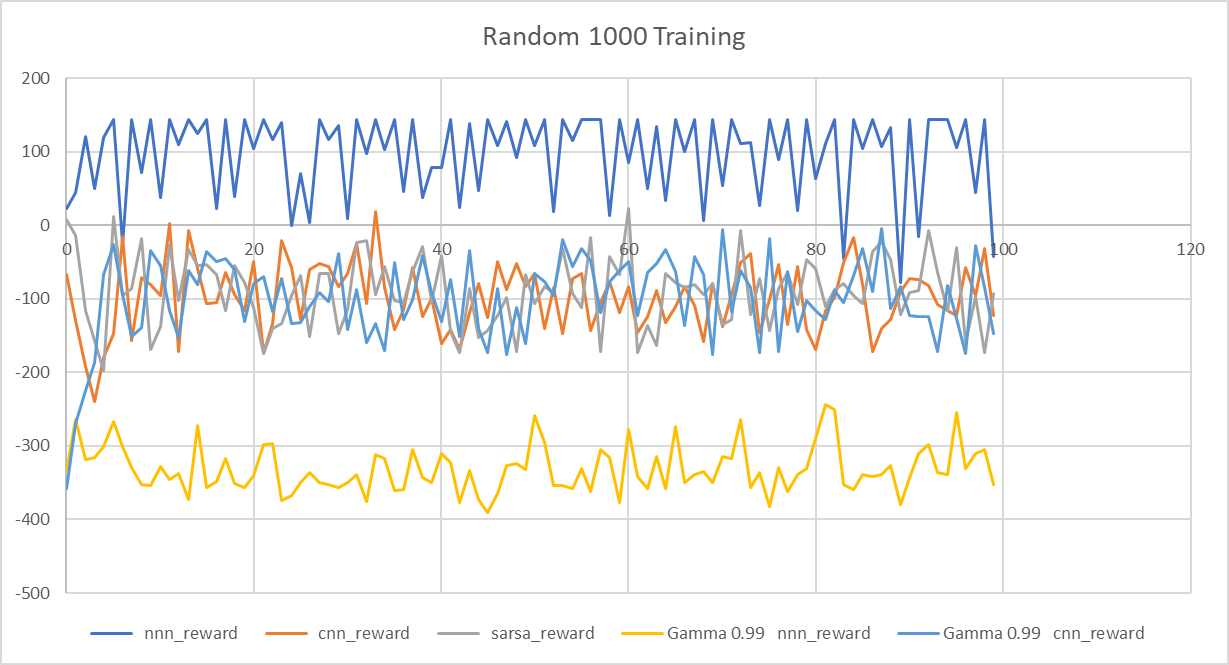
\includegraphics[width=\textwidth]{rand1000.png}
        \caption{Evaluation of models using rand 1000 training scheme. 50 patients randomly changed, variable carb intake, for 1000 iterations}
        \label{fig:rand1000}
    \end{subfigure}
    \caption{Results testing models trained under different conditions on a patient that was unseen during training}
    \label{fig:all_results}
\end{figure}

\section{What I learned?}
I learned a lot about reinforcement learning in general.
I had never seen policy gradient methods (which actor critic is a type of).
Policy gradient methods learn a parameterized value function instead of learning action value estimates (like Q learning).
In actor-critic methods, the actor learns the policy function and the critic learns the value function.
The policy function (actor) uses a softmax distribution to determine action selection probabilities.
This allows the function to converge to the optimal distribution over time (vs $\epsilon$-greedy which may not select best action).
One other interesting application that these probabilities could be used for is to create a suggestion system.
In medical context, a single action may not be optimal (especially from a black box model) but a system could output the actions with sufficiently high probabilities
to give the user (healthcare professional) different suggested options to choose from.

I had never seen Actor-Critic methods so I had to learn what the framework is.
I then learned how to train an actor-critic model. 
These methods can be very flexible, but I struggled to get it working very well.
I am not sure as to why, I think that the value function is very hard to learn in this context.
This probably impeded the training of the model. 


I overall enjoyed learning about Deep Q-Learning.
I had seen Q-Learning in the AI class, but that was several years ago, and I honestly forgot a decent amount.
I had never used it to train a neural network which was fun to do. 
Neural networks seem to be everywhere, and it was fun to get to play with them and reinforcement learning. 
I learned how to generally approach Q-Learning for a neural net and how to set it up.
The example code that I used did not port very well to my problem, so I ended up digging through lots of the exact steps in the learning process.
In this, I also gained some exposure to tensor math, my tensors often had dimensions that did not match what was required.
I freely admit that this was solved primarily by guess-and-check, but I still learned a bit of what operations do and how to think about tensors and their shapes. 

Similarly for SARSA, I had forgotten a lot from seeing it in the AI class. 
I had also not applied it to learn neural networks.
For SARSA, I was never able to find example code training a neural network, so I got to get dirty and build it from scratch.
This also helped me learn how to interface these algorithms to neural nets. 

I implemented a CNN with Q-Learning mostly because it seemed like fun.
I had seen many findings applying CNNs to different problems, and I had never used them before.
Now I would say that I have a basic idea of how they work. 
It was fun to use it on a 1D problem, because most of the pages online are for 2D convolutional networks, 
so I had to figure more out as I go and make more connections.

From the results, I learned that this is a hard problem. Neural nets are not magic and creating the right architecture and using the right hyperparameters 
is very hard to determine. 
They also take a lot of iterations to learn. This was a major limitation of the setup since the MATLAB code was very slow, on the CPU, and cannot be multithreaded.
So training iterations takes a very long time. 

I also learned how to do pytorch. While it isn't strictly educational in the sense of learning new theoretical approaches.
pytorch is still a very common library for machine learning development and it is good to have exposure to the library moving forward.

What are the next steps in this project? Mainly to get the training working. 
Which is a very broad and lofty goal.
One plan is to use the free time over break to allow a computer to train for a long time.
This allows more iterations and hopefully the model will better learn.
Along with this, the $\epsilon$ parameter will decay more slowly over time, to encourage more exploration early.
Another potential method for Q-Learning is to add simulated actions.
Given the problem nature, if we return to a state with a given basal and carb we can expect the same reward.
So we can augment the by adding these simulated actions going to states we have already visited.
For example the opposite action is likely to take us back to the state we were just in.
So including these in the memory could speed up training as it requires fewer transitions to be made in the simulator
which is very slow.
Another parameter to change would be $\gamma$ and the loss function in general.
We want to focus more on near term rewards, so we can set $\gamma$ to an even smaller value. 

\singlespacing
\bibliographystyle{plain}
\bibliography{refs}

\end{document}